%%%%%%%%%%%%%%%%%%%%%%%%%%%%%%%%%%%%%%%%%%%%%%%%%%%%%%%%%%%%%%%%%%%%%%%%
%                                                                      %
%     File: Thesis_Conclusions.tex                                     %
%     Tex Master: Thesis.tex                                           %
%                                                                      %
%     Author: Andre C. Marta                                           %
%     Last modified :  4 Mar 2024                                      %
%                                                                      %
%%%%%%%%%%%%%%%%%%%%%%%%%%%%%%%%%%%%%%%%%%%%%%%%%%%%%%%%%%%%%%%%%%%%%%%%

\chapter{Future Work and Timeline}
\label{chapter:conclusions}

This chapter outlines the work to be carried out during the dissertation period and presents a structured timeline for its development.

% ----------------------------------------------------------------------
\section{Future Work}
\label{section:achievements}

This work established a basis for the dissertation through the implementation and ideal simulation of a tethered \gls{uav} controller. Building on this foundation, the framework will be extended to the full cooperative system and improved to allow testing under more realistic conditions.

A \gls{usv} model will be developed, including an anchor point located on board. This model will be integrated into the \gls{nmpc} formulation. The behaviour of the coupled system will be tested using ideal closed-loop simulations.

The model equations and control parameters will be refined for a specific \gls{uav}, \gls{usv}, and tether hardware configuration. The system dynamics will also be extended to include time-varying external disturbances such as wind and waves. The resulting models will be validated and iteratively improved using simulation or experimental data. The refined and more complete models will then be integrated into the \gls{nmpc} framework.

The convergence rate and optimality of the \gls{nmpc} solutions will be analysed, with particular attention to feasibility and solver performance. A state observer based on an Extended Kalman Filter \cite{simonOptimalStateEstimation2006} may be used to combine model predictions with sensor measurements, providing more accurate and consistent state estimates for the NMPC. Different control modes will be tuned to handle distinct manoeuvres and mission phases.

The controller will be tested in non-ideal simulation environments using more accurate and realistic models. The performance will be evaluated in terms of tracking accuracy, stability, and disturbance rejection. The computational complexity of the \gls{nmpc} optimisation problem will be analysed by assessing solver execution times and convergence behaviour, to determine whether the control problem can be reliably solved at the intended control update frequency, evaluating feasibility for real-time implementation.



% In this work, the problem to be addressed and the associated challenges were defined. The various components involved in the control of an autonomous system were analysed, along with a review of related research, in order to identify the most suitable approach for addressing the proposed challenge.

% After selecting the methodologies to be explored, they were theoretically formulated and applied to a simplified modelling hypothesis of a tethered UAV subsystem. A first version of a nonlinear model predictive controller (NMPC) was developed to generate acceleration control actions corresponding to the thrust magnitude and direction, from which the desired attitude is also derived.

% The controller was implemented in \texttt{Python} using the \texttt{CasADi} framework and tested in closed-loop simulations to evaluate its behaviour and performance. The results demonstrated successful trajectory tracking while respecting all imposed system constraints throughout the simulation.

% This work establishes a solid foundation for the continued development of the system throughout the dissertation, in which the USV will be incorporated, and both the modelling and control framework will be refined, with the ultimate goal of achieving applicability in a real cooperative platform.



% ----------------------------------------------------------------------
\section{Calendar}
\label{section:future}

Figure~\ref{fig:gantt} presents the main tasks planned for the dissertation and their corresponding timeline, organised in a Gantt chart \cite{ganttOrganizingWork1974}.

\begin{sidewaysfigure}
    \centering
    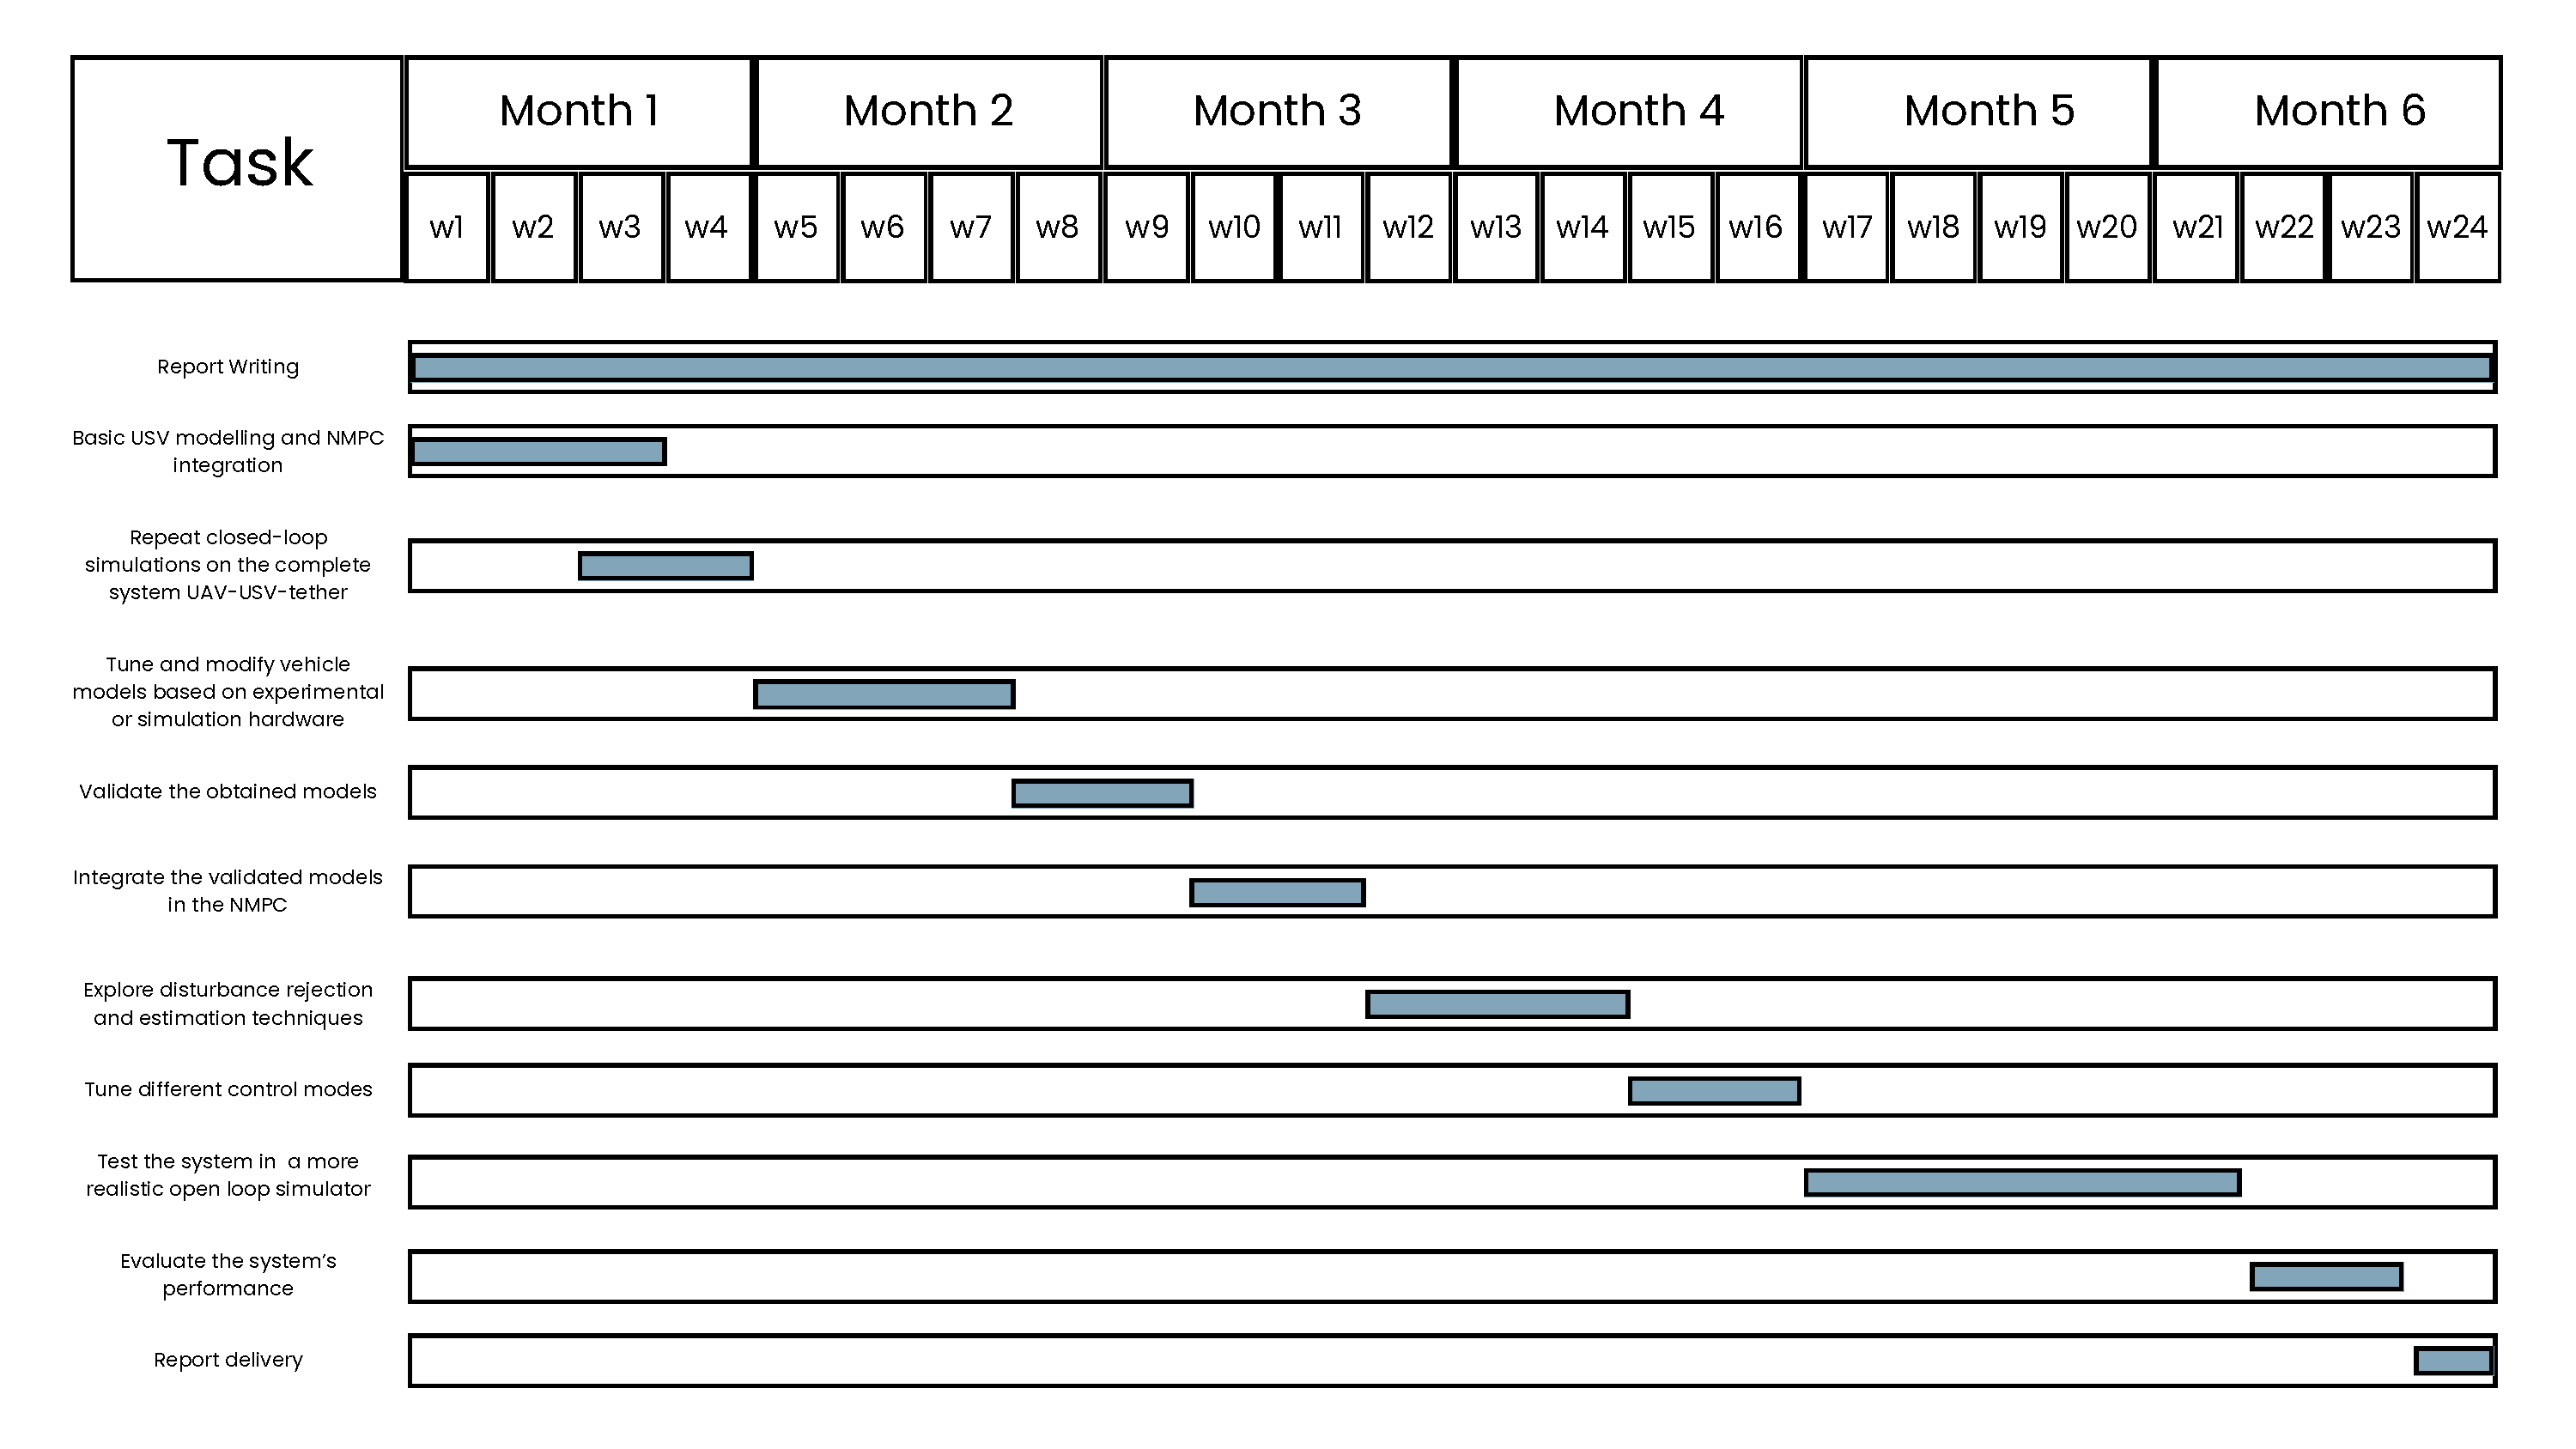
\includegraphics[width=\textheight]{Figures/conclusions/gantt.pdf}
    \caption{Gantt chart containing the task calendarisation for the dissertation period.}
    \label{fig:gantt}
\end{sidewaysfigure}

